\documentclass[xcolor=table]{beamer}
\useoutertheme{progress}
%\usepackage{xcolor}
\usepackage{ragged2e}

\usepackage{eurosym}
\usepackage[T1]{fontenc}
\usepackage{pythontex}
\usepackage{hhline}
\usepackage{array,booktabs}
\newcolumntype{M}[1]{>{\centering\arraybackslash}m{#1}}
\usepackage{caption}
\usepackage{makecell}
\usepackage{lipsum}
\usepackage{pifont}
\usepackage{amssymb}
\usepackage{amsmath}
\usepackage[utf8]{inputenc}
\usepackage[italian]{babel}
\usepackage{graphicx}
\graphicspath{ {./images/} }
\usepackage{spverbatim}
\usepackage{float}
\usepackage{url}
\usepackage{xstring}
\usepackage{hyperref}
\usepackage{upquote}
\definecolor{linkcolor}{RGB}{51,51,179}
\hypersetup{
    colorlinks,
    citecolor=black,
    filecolor=black,
    linkcolor=linkcolor,
    urlcolor=blue
}
\usepackage{fancyvrb,newverbs,xcolor}
\definecolor{cverbbg}{gray}{0.93}
\definecolor{cellcolor}{RGB}{135,206,249}
\usepackage{xifthen}
\usepackage{multirow}
\usepackage{adjustbox}
% following restart section enumeration in different \part
\usepackage{chngcntr}
\counterwithin*{section}{part}

\usepackage{listings}
\lstset{
  basicstyle=\scriptsize\ttfamily,
  backgroundcolor=\color{cverbbg},
  breaklines=true,
  frame=lines,
  framerule=1pt,
  numbers=left,
  numbersep=10pt, 
  keywordstyle=\color{blue},
  commentstyle=\color{green!60!black},
  stringstyle=\color{red},
  showstringspaces=false,  
  framextopmargin=1.5ex,
  framexbottommargin=1.5ex,
  framexleftmargin={\dimexpr 1.5em+3pt},
  xleftmargin={\dimexpr 1.5em+3pt},
  linewidth={\dimexpr \linewidth-3pt},
}



\newcommand{\makesub}[1]{%
  \saveexpandmode\noexpandarg
  \StrSubstitute{#1}{\_}{_}[\temp]%
  \restoreexpandmode%
}

\newcommand{\target}[1]{%
  \makesub{#1}%
  \hypertarget{\temp}{}%
}

\newcommand{\attach}[1]{%
  \makesub{#1}%
  \hyperlink{\temp}{\emph{#1}}%
}
\newcommand{\attachcode}[1]{%
  \makesub{#1}%
  \hyperlink{\temp}{\code{#1}}%
}

\newcommand{\code}[1]{\colorbox{cverbbg}{\texttt{\StrSubstitute{#1}{_}{\_}}}}

\newcommand{\linux}{\textit{Linux}}
\newcommand{\win}{\textit{Windows}}
\newcommand{\nota}[1]{\textbf{Nota}: #1}
\newcommand{\memo}[1]{\textbf{Memo}: #1}
\newcommand{\esempio}[1]{\textbf{Esempio}: #1}
\newcommand{\tbs}{\textbackslash}
\newcommand{\Null}{\code{NULL}}
\newcommand{\api}{\emph{API}}
\newcommand{\key}[1]{\texttt{\StrSubstitute{#1}{_}{\_}}}
\newcommand{\eur}[1]{$\mbox{\euro}$}
\newcommand{\paramtable}[2][]{%
\ifthenelse{\isempty{#2}} {\input{|"/home/luca/latex_scripts/generate_param_table.py '#1'"}} {\input{|"/home/luca/Scrivania/MA/homeworks/homework-04/report/scripts/generate_param_table.py '#1' '#2'"}}%
}
\newcommand{\image}[1]{\input{|"/home/luca/latex_scripts/add_image.py '#1'"}}


\newcommand{\hr}[0]{\begin{center}%
\line(1,0){450}%
\end{center}%
}

\newcommand{\xmark}[0]{\ding{55}}
\newcommand{\vmark}[0]{$\checkmark$}

\newenvironment{myverb}
 {\SaveVerbatim{cverb}}
 {\endSaveVerbatim
  \flushleft\fboxrule=0pt\fboxsep=.5em
  \colorbox{cverbbg}{%
    \makebox[\dimexpr\linewidth-2\fboxsep][l]{\BUseVerbatim{cverb}}%
  }
  \endflushleft
}


% justify in itemize
\makeatletter
\renewcommand{\itemize}[1][]{%
  \beamer@ifempty{#1}{}{\def\beamer@defaultospec{#1}}%
  \ifnum \@itemdepth >2\relax\@toodeep\else
    \advance\@itemdepth\@ne
    \beamer@computepref\@itemdepth% sets \beameritemnestingprefix
    \usebeamerfont{itemize/enumerate \beameritemnestingprefix body}%
    \usebeamercolor[fg]{itemize/enumerate \beameritemnestingprefix body}%
    \usebeamertemplate{itemize/enumerate \beameritemnestingprefix body begin}%
    \list
      {\usebeamertemplate{itemize \beameritemnestingprefix item}}
      {\def\makelabel##1{%
          {%
            \hss\llap{{%
                \usebeamerfont*{itemize \beameritemnestingprefix item}%
                \usebeamercolor[fg]{itemize \beameritemnestingprefix item}##1}}%
          }%
        }%
      }
  \fi%
  \beamer@cramped%
  \justifying% NEW
  %\raggedright% ORIGINAL
  \beamer@firstlineitemizeunskip%
}
\makeatother



\setbeamercolor{background canvas}{bg=white}
\setbeamercolor{frametitle}{bg=footlinecolor!20}
\usepackage[T1]{fontenc}
\usepackage[utf8]{inputenc}
\usepackage{pgfpages}
%\setbeameroption{show notes on second screen}
\usepackage[absolute,overlay]{textpos}

\newcommand{\noindentitemize}[0]{
\settowidth{\leftmargini}{\usebeamertemplate{itemize item}}%
\addtolength{\leftmargini}{\labelsep}%
}


\AtBeginSubsection[]
{
	
	\begingroup
    \frame[c,noframenumbering]{
    \begin{beamercolorbox}[sep=12pt,center]{part title}
    \tableofcontents[currentsubsection, 
    hideothersubsections, 
    sectionstyle=show/shaded, 
    subsectionstyle=show/shaded, 
    ]
    \end{beamercolorbox}
    }
    
    \endgroup
    		
}

\setbeamertemplate{frametitle}[default][center]





\begin{document}
\addtocounter{framenumber}{1}

\title{Progetto \textit{Performance Modeling of Computer Systems and Networks\\a.a: 2022/2023}}
\author{Luca Mastrobattista\\0292461}
\date{}
\begin{frame}[c,noframenumbering]
\titlepage

\end{frame}

%*************************************************************************
\section{Introduzione}
\begin{frame}{Caso di studio}
\justifying
Si prende in esame il contesto di un locale che offre servizi di bar e pizzeria in un piccolo paese.
\begin{itemize}
\item si analizza la gestione delle richieste in un'intera giornata lavorativa, sia nei giorni settimanali che finesettimanali

\item il locale è aperto dalle 7.00 alle 15.00 e dalle 18.00 alle 2.00

\end{itemize}
\end{frame}



\begin{frame}{Obiettivi}
\begin{itemize}
\item Rispettare dei servizi di qualità:
\begin{itemize}
\item[-] Limitare i tempi di risposta per le richieste al bar a 3 minuti
\item[-] Limitare i tempi di risposta per le richieste alla pizzeria a 10 minuti
\end{itemize}

\item Massimizzare i guadagni cercando il numero di serventi ottimali 
\end{itemize}
\end{frame}


\section{Modello concettuale}
\begin{frame}{Visualizzazione grafica}\justifying
\begin{figure}[H]
\centering
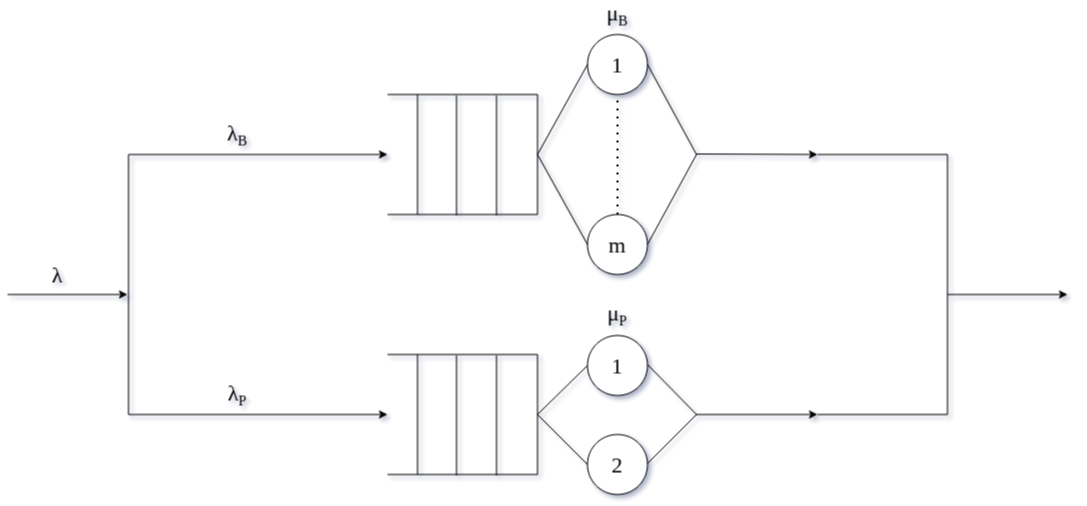
\includegraphics[scale=0.2]{conceptual_model}
\end{figure}
\begin{itemize}
\item La frequenza di arrivo $\lambda$ si compone della frequenza di arrivo $\lambda_B$ e $\lambda_P$ 
\item Ogni servente di tipo B rappresenta un barista assunto, che lavora con una frequenza $\mu_B$
\item Ogni servente di tipo P, invece, rappresenta una delle due richieste che il pizzaiolo è in grado di gestire contemporaneamente e lavora con frequenza $\mu_P$
\end{itemize}
\end{frame}

\begin{frame}{Eventi e variabili di stato}\justifying
\begin{itemize}
\item Eventi
\begin{itemize}
\item[-] Arrivi dall'esterno
\item[-] Completamenti
\end{itemize}

\item[]

\item Completamenti
\begin{itemize}
\item[-] Numero di richieste di tipo B al centro
\item[-] Numero di richieste di tipo P al centro
\item[-] Stato del servente, per ogni servente di tipo B e P
\end{itemize}
\end{itemize}
\end{frame}


\section{Modello delle specifiche}
\begin{frame}{Distribuzione degli arrivi}\justifying

\begin{itemize}
\item Distribuzione base: Gli arrivi sono assunti esponenziali, per offrire una flessibilità dei tempi di interarrivo che riflette accuratamente la casualità degli arrivi in un bar.

\item Ritardo gaussiano: È stato poi introdotto un ritardo gaussiano per rendere il modello più realistico permettendo di tener conto di effetti come le ore punta.
\end{itemize}
\bigskip

\begin{adjustbox}{width=\textwidth}
\begin{tabular}{ |c|c|c|c|c|c|c|c|c| }
\hline
\cellcolor{cellcolor}Fascia oraria & \cellcolor{cellcolor}$\lambda${\textsubscript{B,W}} & \cellcolor{cellcolor}$\lambda${\textsubscript{P,W}} & \cellcolor{cellcolor} $\lambda_{B,WE}$ & \cellcolor{cellcolor} $\lambda_{P,WE}$ & \cellcolor{cellcolor} $\mu_B$ & \cellcolor{cellcolor} $\sigma_B$ & \cellcolor{cellcolor} $\mu_P$ & \cellcolor{cellcolor} $\sigma_P$ \\
\hline
\hline
07:00 $\rightarrow$ 11:00 & 30 j/h & \xmark & 30 j/h & \xmark & 8 & 1.2 & \xmark & \xmark \\
\hline
11:00 $\rightarrow$ 15:00 & 12.5 j/h & \xmark & 20 j/h & \xmark & 13.5 & 2 & \xmark & \xmark \\
\hline
\hline
18:00 $\rightarrow$ 19:00 & 25 j/h & \xmark & 45 j/h & \xmark & 18.5 & 0.4 & \xmark & \xmark \\
\hline
19:00 $\rightarrow$ 23:00 & 12.5 j/h & 10 j/h & 22.5 j/h & 30 j/h & 22.5 & 2 & 20.5 & 1 \\
\hline
23:00 $\rightarrow$ 02:00 & 10 j/h & \xmark & 20 j/h & \xmark & 24 & 0.9 & \xmark & \xmark \\
\hline
\end{tabular} 
\end{adjustbox}
\end{frame}

\begin{frame}{Tempi di servizio}\justifying
I tempi di servizio si assumono esponenziali per entrambi i tipi di serventi.
\begin{itemize}
\item Servente di tipo B: Si assume che ogni servente sia in grado di completare una richiesta con il tempo medio di 2 minuti, durante i quali si dedica esclusivamente a quella richiesta.

\item Servente di tipo P: Si assume che ogni pizza posso essere completamente preparata con un tempo medio di 3 minuti.
\end{itemize}
\end{frame}

\begin{frame}{Guadagni e costi}\justifying
\begin{itemize}
\item Guadagni
\begin{itemize}
\item[-] Per ogni richiesta di tipo B si assume un guadagno medio di 5,00 $\mbox{\euro}$

\item[-] Per ogni richiesta di tipo P si assume un guadagno medio di 10,00 $\mbox{\euro}$
\end{itemize}

\item Costi
\begin{itemize}
\item[-] Stipendio medio di un barista per 8 ore: 40,00 $\mbox{\euro}$
\item[-] Stipendio del pizzaiolo per giorno: 50,00 $\mbox{\euro}$
\item[-] Costo medio delle bollette: 2.750,00 \eur{} al mese
\item[-] Costo medio dell'affitto: 1.500,00 \eur{} al mese
\item[-] Costo medio per il rifornimento: 2.000,00 \eur{} al mese
\end{itemize}
\end{itemize}
\end{frame}


\section{Modello computazionale}

\begin{frame}{Descrizione generale del programma}\justifying
Il simulatore, implementato in \textit{Python}, segue l'approccio della \textit{next-event simulation} ed è altamente configurabile in base alle esigenze, specificando opportuni flag a riga comando:

\begin{figure}[H]
\centering
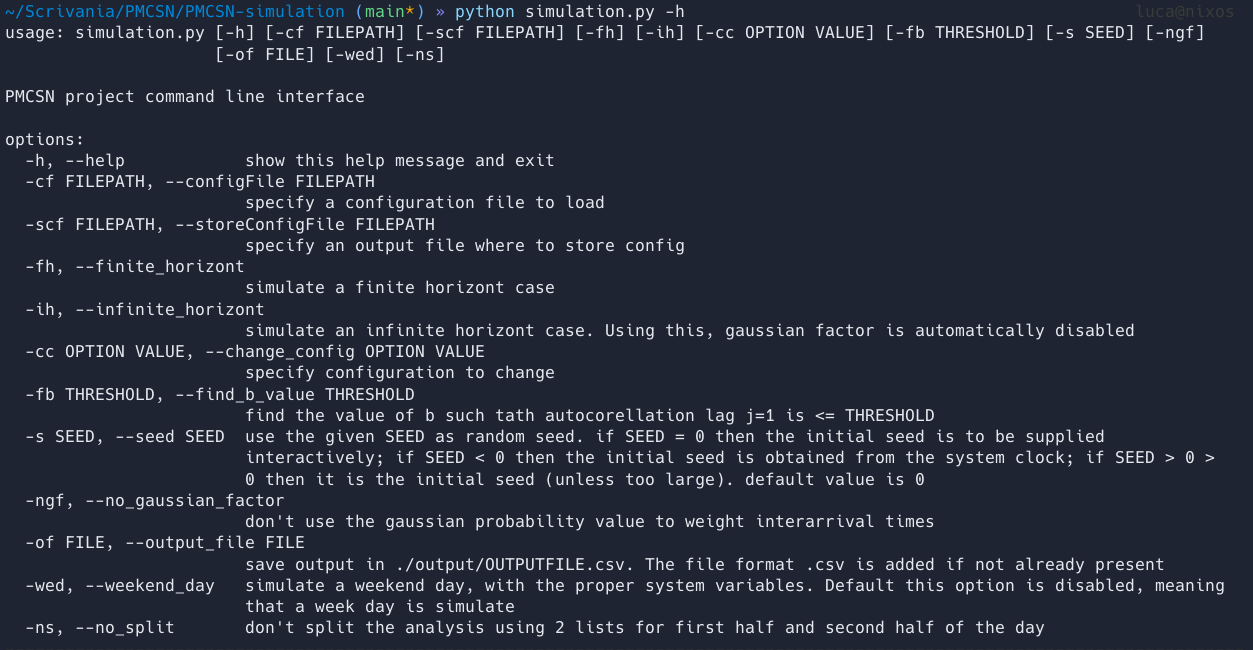
\includegraphics[scale=0.2]{program_help}
\end{figure}
\end{frame}

\begin{frame}{Politica di scelta del servente}\justifying
La scelta del servente per gestire una nuova richiesta è diversa per i due tipi B e P:
\begin{itemize}
\item Richieste al bar: La scelta del prossimo servente segue la politica di \textit{equity}
\item Richieste alla pizzeria: Il prossimo servente selezionato è il primo trovato libero scandendo la lista in ordine crescente
\end{itemize}
\end{frame}

\begin{frame}[fragile]{Evento di campionamento}
\justifying
Il tempo del prossimo evento di campionamento viene impostato in modo da evitare che due eventi successivi siano entrambi eventi di campionamento:

\begin{lstlisting}[language=Python, firstnumber=242, title=\key{simulation.py}, tabsize=3,framexleftmargin={\dimexpr 1.5em+15pt}, xleftmargin={\dimexpr 1.5em+15pt},]
times = []
for index, ev in enumerate(stats.events):
	if index != e and ev.x == 1:
		times.append(ev.t)
stats.events[e].t = min(times) + samplingInterarrivalTime
\end{lstlisting}
\end{frame}


\section{Verifica}

\begin{frame}{Differenza tra risultati teorici e sperimentali}\justifying
Ogni \textit{run} di simulazione con le configurazioni di default produce statistiche sperimentali che sono diverse rispetto a quelle teoriche. Il motivo di tale differenza è che il numero di job processati è piccolo, e perciò le statistiche sperimentali sono poco rappresentative.
\bigskip

\centering
\begin{adjustbox}{scale=0.6}

\begin{tabular}{ |c|c|c|c|c| }
\hline
\cellcolor{cellcolor} \textit{B type} & \multicolumn{2}{c|}{\cellcolor{cellcolor}Week} & \multicolumn{2}{c|}{\cellcolor{cellcolor}Weekend} \\
\hline
\cellcolor{cellcolor}Statistica & \cellcolor{cellcolor}Risultato teorico & \cellcolor{cellcolor}Risultato sperimentale & \cellcolor{cellcolor}Risultato teorico & \cellcolor{cellcolor}Risultato sperimentale \\
\hline
\hline
avgInterarrivals & 3.471 min & 2.984 $\pm$ 0.076 min & 2.413 min & 2.494 $\pm$ 0.025 min \\
\hline
avgWaits & 2.251 min & 2.284 $\pm$ 0.047 min & 2.524 min & 2.266 $\pm$ 0.036 min \\
\hline
avgNumNodes & 0.682 j & 0.788 $\pm$ 0.029 j & 1.102 j & 0.801 $\pm$ 0.021 j  \\
\hline
avgDelays & 0.251 min & 0.268 $\pm$ 0.014 min & 0.524 min & 0.286 $\pm$ 0.010 min \\
\hline
avgNumQueues & 0.106 j & 0.091 $\pm$ 0.008 j & 0.273 j & 0.103 $\pm$  0.005 j \\
\hline
avgService (1) & 2 min & 1.724 $\pm$ 0.047 min & 2 min & 1.772 $\pm$  0.035 min \\
\hline
avgService (2) & 2 min & 2.367 $\pm$ 0.039 min & 2 min & 2.216 $\pm$ 0.036 min \\
\hline
\end{tabular}
\end{adjustbox}
\bigskip

\begin{adjustbox}{scale=0.6}
\centering
\begin{tabular}{ |c|c|c|c|c| }
\hline
\cellcolor{cellcolor} \textit{P type} & \multicolumn{2}{c|}{\cellcolor{cellcolor}Week} & \multicolumn{2}{c|}{\cellcolor{cellcolor}Weekend} \\
\hline
\cellcolor{cellcolor}Statistica & \cellcolor{cellcolor}Risultato teorico & \cellcolor{cellcolor}Risultato sperimentale & \cellcolor{cellcolor}Risultato teorico & \cellcolor{cellcolor}Risultato sperimentale \\
\hline
\hline
avgInterarrivals & 5.882 min & 4.408 $\pm$ 0.160 min & 2.000 min & 1.846 $\pm$ 0.036 min \\
\hline
avgWaits & 3.209 min & 3.465 $\pm$ 0.116 min &  6.857 min & 5.667 $\pm$ 0.151 min \\
\hline
avgNumNodes & 0.545 j & 0.761 $\pm$ 0.042 j & 3.429 j & 2.962 $\pm$ 0.046 j \\
\hline
avgDelays & 0.209 min & 0.050 $\pm$ 0.008 min & 3.857 min & 2.514 $\pm$ 0.083 min \\
\hline
avgNumQueues & 0.035 j & 0.013 $\pm$ 0.003 j & 1.929 j & 1.316 $\pm$ 0.037 j \\
\hline
avgService (1) & 3 min & 2.918 $\pm$ 0.136 min & 3 min & 2.947 $\pm$ 0.116 \\
\hline
avgService (2) & 3 min & 4.722 $\pm$ 0.201 min & 3 min & 3.361 $\pm$ 0.069 min \\
\hline

\end{tabular}
\end{adjustbox}


\end{frame}

\begin{frame}[fragile]{Nuova configurazione: \key{verify1.py}}\justifying
Si definisce il nuovo file di configurazione per cercare di aumentare la rappresentatività delle statistiche:
\begin{lstlisting}[language=Python, numbers=none, title=\key{configurations/verify1.py}]
# per esprimere i tempi in secondi:
SLOTSTIME = [ (i * 3600) for i in [7, 11, 15, 18, 19, 23] ] 
STOP_B = 26 * 3600   
# per rendere il sistema stabile anche dal punto di vista analitico
MEAN_SERVICE_TIME_B = 0.5
MEAN_SERVICE_TIME_P = 0.5
# i lambda:
WEEK_LAMBDA_B = [2, 2, 0, 3, 3, 3]
WEEK_LAMBDA_P = 1.7
\end{lstlisting}
\end{frame}

\begin{frame}{\key{verify1.py} - Risultati}\justifying
Eseguendo il comando \key{python simulation.py -s 123 -ngf -cf configurations/verify1.py}, si ottengono i seguenti risultati:
\bigskip

\begin{minipage}{0.5\textwidth}
\centering
\begin{adjustbox}{scale=0.5}
\begin{tabular}{ |c|c|c| }
\hline
\cellcolor{cellcolor} \textit{B type} & \multicolumn{2}{c|}{\cellcolor{cellcolor}Week} \\
\hline
\cellcolor{cellcolor}Statistica & \cellcolor{cellcolor}Risultato teorico & \cellcolor{cellcolor}Risultato sperimentale \\
\hline
\hline
avgInterarrivals & 0.317 s & 0.466 $\pm$ 0.002 s \\
\hline
avgWaits & 0.415 s & 0.337 $\pm$ 0.000 s \\
\hline
avgNumNodes & 1.394 j & 0.730 $\pm$ 0.001 j \\
\hline
avgDelays & 0.115 s & 0.037 $\pm$ 0.000 s \\
\hline
avgNumQueues & 0.449 j & 0.083 $\pm$ 0.000 j \\
\hline
avgService (1) & 0.3 s & 0.300 $\pm$ 0.000 s \\
\hline
avgService (2) & 0.3 s & 0.300 $\pm$ 0.000 s \\
\hline
\end{tabular}
\end{adjustbox}

\end{minipage}
\begin{minipage}{0.5\textwidth}
\centering
\begin{adjustbox}{scale=0.5}
\begin{tabular}{ |c|c|c| }
\hline
\cellcolor{cellcolor} \textit{P type} & \multicolumn{2}{c|}{\cellcolor{cellcolor}Week} \\
\hline
\cellcolor{cellcolor}Statistica & \cellcolor{cellcolor}Risultato teorico & \cellcolor{cellcolor}Risultato sperimentale \\
\hline
\hline
avgInterarrivals & 0.588 s & 0.593 $\pm$ 0.000 s \\
\hline
avgWaits & 0.610 s & 0.603 $\pm$ 0.000 s \\
\hline
avgNumNodes & 1.037 j & 1.016 $\pm$ 0.000 j \\
\hline
avgDelays & 0.110 s & 0.105 $\pm$ 0.000 s \\
\hline
avgNumQueues & 0.187 j & 0.176 $\pm$ 0.000 j \\
\hline
avgService (1) & 0.5 s & 0.496 $\pm$ 0.000 s \\
\hline
avgService (2) & 0.5 s & 0.501 $\pm$ 0.000 s \\
\hline
\end{tabular}
\end{adjustbox}
\end{minipage}
\bigskip

Si può osservare come i valori teorici per le richieste di tipo "P", che sono state in tutto 24407, cominciano a convergere ai valori teorici. Per le richieste di tipo "B", nonostante siano state 181785, i valori ottenuti sono ancora lontani da quelli teorici.
\end{frame}

\begin{frame}{Possibile spiegazione e mitigazione}\justifying
\begin{itemize}
\item Si può notare che la frequenza di interarrivo media nella prima metà della giornata è più bassa rispetto alla seconda metà e perciò il numero di job processati e i campioni raccolti nelle prime 8 ore saranno inferiori rispetto alle ultime 8 ore.

\item Per mantenere un'analisi media equilibrata, si è introdotta un'opzione predefinita che suddivide l'analisi in due fasce orarie separate. Si raccolgono e si calcolano i dati statistici separatamente per entrambe le metà della giornata. 

\item Le medie e varianze globali si otterranno mediando i risultati ponderati per il numero di job processati.
\end{itemize}
\bigskip

\begin{minipage}{0.5\textwidth}
\[
	\mu_{glob} = \frac{n_1 \mu_1 + n_2 \mu_2}{n_1 + n_2}
\]
\end{minipage}
\begin{minipage}{0.5\textwidth}
\[
	\sigma^2_{glob} = \frac{n_1 \sigma^2_1 + n_2 \sigma^2_2}{n_1 + n_2}
\]
\end{minipage}
\end{frame}

\begin{frame}[fragile]{Nuova opzione - Risultati}\justifying
Con la nuova opzione attiva, lanciando il comando
\begin{lstlisting}[language=Bash, numbers=none, ]
python simulation.py -s 123 -ngf -cf configurations/verify1.py
\end{lstlisting}

si ottengono i seguenti risultati:
\bigskip

\centering
\begin{adjustbox}{scale=0.6}

\begin{tabular}{ |c|c|c| }
\hline
\cellcolor{cellcolor} \textit{B type} & \multicolumn{2}{c|}{\cellcolor{cellcolor}Week} \\
\hline
\cellcolor{cellcolor}Statistica & \cellcolor{cellcolor}Risultato teorico & \cellcolor{cellcolor}Risultato sperimentale \\
\hline
\hline
avgInterarrivals & 0.400 s & 0.399 $\pm$ 0.000 s \\
\hline
avgWaits & 0.353 s & 0.355 $\pm$ 0.000 s \\
\hline
avgNumNodes & 0.894 j & 0.938 $\pm$ 0.000 j \\
\hline
avgDelays & 0.053 s & 0.055 $\pm$ 0.000 s \\
\hline
avgNumQueues & 0.144 j & 0.156 $\pm$ 0.000 j \\
\hline
avgService (1) & 0.3 s & 0.300 $\pm$ 0.000 s \\
\hline
avgService (2) & 0.3 s & 0.299 $\pm$ 0.000 s \\
\hline
\end{tabular}
\end{adjustbox}
\bigskip

Anche per le richieste di tipo "B", adesso i risultati convergono a quelli teorici.
\end{frame}

\begin{frame}[fragile]{Verifica della politica di selezione del server}\justifying
Per valutare la politica di selezione è stato eseguito il seguente comando:
\begin{lstlisting}[language=Bash, numbers=none, ]
python simulation.py -s 123 -ngf -cf configurations/verify1.py -cc servers_b 10 -cc servers_p 10
\end{lstlisting}

I risultati ottenuti da questa configurazione sono riportati di seguito:
\vspace*{0.1ex}
	
\hspace*{\fill}
\begin{minipage}{0.4\textwidth}
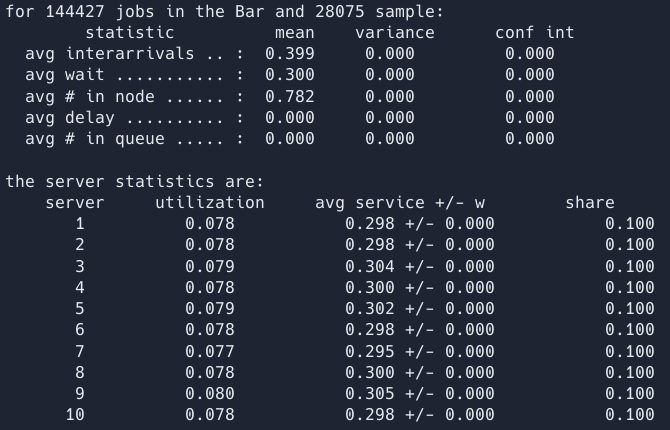
\includegraphics[width=\textwidth]{rho_services_b}
\end{minipage}
\hfill
\begin{minipage}{0.4\textwidth}
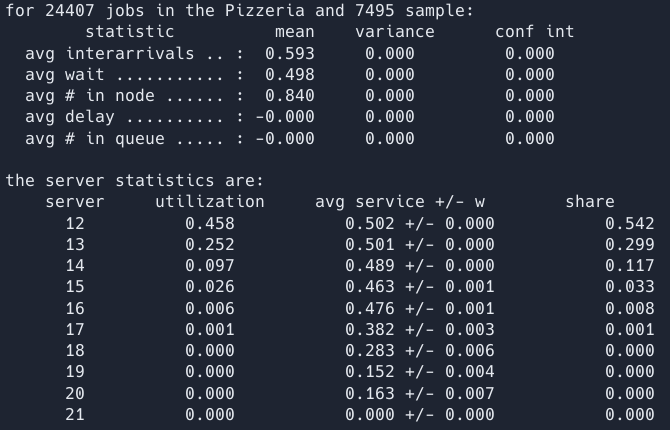
\includegraphics[width=\textwidth]{rho_services_p}
\end{minipage}
\hspace*{\fill}
\bigskip

Tutti i server di tipo "B" presentano valori simili per utilizzazione, tempo di servizio e share, mentre per i server di tipo "P" c'è un decremento dei valori all'aumentare dell'indice del server.
\end{frame}

\section{Validazione}

\begin{frame}{Problematiche riscontrate}\justifying
\begin{itemize}
\item Durante il processo di validazione si sono riscontrate delle sfide significative nell'utilizzo dell'analisi a orizzonte finito, principalmente dovute al numero limitato di job processati. Questa limitazione ha comportato un campione statistico ridotto e, di conseguenza, una maggiore variabilità nei risultati osservati.

\item Per validare il modello, quindi, si è deciso di adottare un'analisi a orizzonte infinito in modo da ottenere risultati più stabili. In questa fase verifichiamo se, per ciascuna fascia oraria, le statistiche generate dal nostro simulatore convergono ai valori reali. 
\end{itemize}
\end{frame}

\begin{frame}{Analisi a orizzonte infinito}\justifying
\begin{itemize}
\item Utilizzando \key{k = 128} batches, ciascuno con \key{b = 1024} campioni, l'autocorrelazione per lag \texttt{j = 1} è inferiore a \key{0.2}, contribuendo così alla stabilità e all'affidabilità dei risultati.
\item L'analisi viene condotta per ciascun tipo di richiesta e per ciascuna statistica di interesse, coprendo tutte le fasce orarie sia nei giorni lavorativi che nei giorni del fine settimana.
\end{itemize}
\end{frame}

\begin{frame}{Interarrivi - bar}
\justifying
\begin{adjustbox}{width=\textwidth}
\centering
\begin{tabular}{ |c|c|c|c|c|c|c| }
\cline{2-6}
\multicolumn{1}{c}{} & \multicolumn{5}{|c|}{\cellcolor{cellcolor}\textit{B type - Interarrivals}}\\
\cline{2-6}
\multicolumn{1}{c|}{} & \cellcolor{cellcolor}Slot & \cellcolor{cellcolor}Risultato teorico & \cellcolor{cellcolor}Risultato sperimentale &  \cellcolor{cellcolor}Media nell'intervallo &
\cellcolor{cellcolor}Errore \\
\cline{2-6}
\noalign{\vspace{0.5ex}}
\hline
\cellcolor{cellcolor}& 0 & 2.000 min & 2.000 $\pm$ 0.014 min & \checkmark & \\ 
\cline{2-6}
\cellcolor{cellcolor}& 1 & 4.762 min & 4.950 $\pm$ 0.389 min & \checkmark & \\
\cline{2-6}
\cellcolor{cellcolor}& 3 & 2.381 min & 2.614 $\pm$ 0.477 min & \checkmark & \\
\cline{2-6}
\cellcolor{cellcolor}& 4 & 4.762 min & 5.154 $\pm$ 0.811 min & \checkmark & \\
\cline{2-6}
\multirow{-6}{*}{\rotatebox[origin=c]{90}{\cellcolor{cellcolor}Week}} & 5 & 5.882 min & 6.217 $\pm$ 0.074 min & \checkmark & \\
\hline
\hline
\cellcolor{cellcolor}& 0 & 2.000 min & 2.000 $\pm$ 0.014 min & \checkmark & \\ 
\cline{2-6}
\cellcolor{cellcolor}& 1 & 2.941 min & 3.091 $\pm$ 0.322 min & \checkmark & \\
\cline{2-6}
\cellcolor{cellcolor}& 3 & 1.333 min & 1.460 $\pm$ 0.259 min & \checkmark & \\
\cline{2-6}
\cellcolor{cellcolor}& 4 & 2.667 min & 2.794 $\pm$ 0.268 min & \checkmark & \\
\cline{2-6}
\multirow{-6}{*}{\rotatebox[origin=c]{90}{\cellcolor{cellcolor}Weekend}} & 5 & 2.941 min & 3.065 $\pm$ 0.285 min & \checkmark & \\
\hline
\end{tabular}
\end{adjustbox}
\end{frame}


\begin{frame}{Interarrivi al bar - Immagini \textit{week}}\justifying
\centering
\includegraphics[width=0.4\textwidth]{/infinite/slot_0/avgInterarrivals/week_B_0}
\includegraphics[width=0.4\textwidth]{/infinite/slot_1/avgInterarrivals/week_B_1}
\includegraphics[width=0.4\textwidth]{/infinite/slot_3/avgInterarrivals/week_B_3}
\includegraphics[width=0.4\textwidth]{/infinite/slot_4/avgInterarrivals/week_B_4}
\includegraphics[width=0.4\textwidth]{/infinite/slot_5/avgInterarrivals/week_B_5}
\end{frame}


\begin{frame}{Interarrivi al bar - Immagini \textit{weekend}}\justifying
\centering
\includegraphics[width=0.4\textwidth]{/infinite/slot_0/avgInterarrivals/weekend_B_0}
\includegraphics[width=0.4\textwidth]{/infinite/slot_1/avgInterarrivals/weekend_B_1}
\includegraphics[width=0.4\textwidth]{/infinite/slot_3/avgInterarrivals/weekend_B_3}
\includegraphics[width=0.4\textwidth]{/infinite/slot_4/avgInterarrivals/weekend_B_4}
\includegraphics[width=0.4\textwidth]{/infinite/slot_5/avgInterarrivals/weekend_B_5}
\end{frame}

\begin{frame}{Tempi di risposta - bar}\justifying
\begin{adjustbox}{width=\textwidth}
\centering
\begin{tabular}{ |c|c|c|c|c|c| }
\cline{2-6}
\multicolumn{1}{c}{} & \multicolumn{5}{|c|}{\cellcolor{cellcolor}\textit{B type - Waits}}\\
\cline{2-6}
\multicolumn{1}{c|}{} & \cellcolor{cellcolor}Slot & \cellcolor{cellcolor}Risultato teorico & \cellcolor{cellcolor}Risultato sperimentale &  \cellcolor{cellcolor}Media nell'intervallo &
\cellcolor{cellcolor}Errore \\
\cline{2-6}
\noalign{\vspace{0.5ex}}
\hline
\cellcolor{cellcolor}& 0 & 2.667 min & 2.665 $\pm$ 0.035 min & \checkmark & \\ 
\cline{2-6}
\cellcolor{cellcolor}& 1 & 2.092 min & 2.083 $\pm$ 0.018 min & \checkmark & \\ 
\cline{2-6}
\cellcolor{cellcolor}& 3 & 2.428 min & 2.440 $\pm$ 0.027 min & \checkmark & \\ 
\cline{2-6}
\cellcolor{cellcolor}& 4 & 2.092 min & 2.086 $\pm$ 0.021 min & \checkmark & \\ 
\cline{2-6}
\multirow{-6}{*}{\rotatebox[origin=c]{90}{\cellcolor{cellcolor}Week}} & 5 & 2.060 min & 2.067 $\pm$ 0.023 min & \checkmark & \\ 
\hline
\hline
\cellcolor{cellcolor}& 0 & 2.667 min & 2.665 $\pm$ 0.035 min & \checkmark & \\ 
\cline{2-6}
\cellcolor{cellcolor}& 1 & 2.261 min & 2.257 $\pm$ 0.024 min & \checkmark & \\ 
\cline{2-6}
\cellcolor{cellcolor}& 3 & 4.571 min & 4.499 $\pm$ 0.115 min & \checkmark & \\ 
\cline{2-6}
\cellcolor{cellcolor}& 4 & 2.327 min & 2.339 $\pm$ 0.031 min & \checkmark & \\ 
\cline{2-6}
\multirow{-6}{*}{\rotatebox[origin=c]{90}{\cellcolor{cellcolor}Weekend}} & 5 & 2.261 min & 2.246 $\pm$ 0.025 min & \checkmark & \\ 
\hline
\end{tabular}
\end{adjustbox}

\end{frame}

\begin{frame}{Tempi di risposta al bar - Immagini \textit{week}}\justifying
\centering
\includegraphics[width=0.4\textwidth]{/infinite/slot_0/avgWaits/week_B_0}
\includegraphics[width=0.4\textwidth]{/infinite/slot_1/avgWaits/week_B_1}
\includegraphics[width=0.4\textwidth]{/infinite/slot_3/avgWaits/week_B_3}
\includegraphics[width=0.4\textwidth]{/infinite/slot_4/avgWaits/week_B_4}
\includegraphics[width=0.4\textwidth]{/infinite/slot_5/avgWaits/week_B_5}
\end{frame}

\begin{frame}{Tempi di risposta al bar - Immagini \textit{weekend}}\justifying
\centering
\includegraphics[width=0.4\textwidth]{/infinite/slot_0/avgWaits/weekend_B_0}
\includegraphics[width=0.4\textwidth]{/infinite/slot_1/avgWaits/weekend_B_1}
\includegraphics[width=0.4\textwidth]{/infinite/slot_3/avgWaits/weekend_B_3}
\includegraphics[width=0.4\textwidth]{/infinite/slot_4/avgWaits/weekend_B_4}
\includegraphics[width=0.4\textwidth]{/infinite/slot_5/avgWaits/weekend_B_5}
\end{frame}



\begin{frame}{Numero di richieste nel centro - bar}\justifying
\begin{adjustbox}{width=\textwidth}
\centering
\begin{tabular}{ |c|c|c|c|c|c| }
\cline{2-6}
\multicolumn{1}{c}{} & \multicolumn{5}{|c|}{\cellcolor{cellcolor}\textit{B type - Num. in the nodes}}\\
\cline{2-6}
\multicolumn{1}{c|}{} & \cellcolor{cellcolor}Slot & \cellcolor{cellcolor}Risultato teorico & \cellcolor{cellcolor}Risultato sperimentale &  \cellcolor{cellcolor}Media nell'intervallo &
\cellcolor{cellcolor}Errore \\
\cline{2-6}
\noalign{\vspace{0.5ex}}
\hline
\cellcolor{cellcolor}& 0 & 1.333 min & 1.336 $\pm$ 0.021 min & \checkmark & \\ 
\cline{2-6}
\cellcolor{cellcolor}& 1 & 0.439 min & 0.440 $\pm$ 0.006 min & \checkmark & \\
\cline{2-6}
\cellcolor{cellcolor}& 3 & 1.020 min & 1.031 $\pm$ 0.016 min & \checkmark & \\
\cline{2-6}
\cellcolor{cellcolor}& 4 & 0.439 min & 0.440 $\pm$ 0.007 min & \checkmark & \\
\cline{2-6}
\multirow{-6}{*}{\rotatebox[origin=c]{90}{\cellcolor{cellcolor}Week}} & 5 & 0.350 min & 0.355 $\pm$ 0.005 min & \checkmark & \\
\hline
\hline
\cellcolor{cellcolor}& 0 & 1.333 min & 1.336 $\pm$ 0.021 min & \checkmark & \\ 
\cline{2-6}
\cellcolor{cellcolor}& 1 & 0.769 min & 0.773 $\pm$ 0.011 min & \checkmark & \\
\cline{2-6}
\cellcolor{cellcolor}& 3 & 3.429 min & 3.399 $\pm$ 0.095 min & \checkmark & \\
\cline{2-6}
\cellcolor{cellcolor}& 4 & 0.873 min & 0.881 $\pm$ 0.014 min & \checkmark & \\
\cline{2-6}
\multirow{-6}{*}{\rotatebox[origin=c]{90}{\cellcolor{cellcolor}Weekend}} & 5 & 0.769 min & 0.769 $\pm$ 0.011 min & \checkmark & \\
\hline
\end{tabular}
\end{adjustbox}
\end{frame}

\begin{frame}{Numero di richieste nel centro al bar - Immagini \textit{week}}\justifying
\centering
\includegraphics[width=0.4\textwidth]{/infinite/slot_0/avgNumNodes/week_B_0}
\includegraphics[width=0.4\textwidth]{/infinite/slot_1/avgNumNodes/week_B_1}
\includegraphics[width=0.4\textwidth]{/infinite/slot_3/avgNumNodes/week_B_3}
\includegraphics[width=0.4\textwidth]{/infinite/slot_4/avgNumNodes/week_B_4}
\includegraphics[width=0.4\textwidth]{/infinite/slot_5/avgNumNodes/week_B_5}
\end{frame}
\begin{frame}{Numero di richieste nel centro al bar - Immagini \textit{weekend}}\justifying
\centering
\includegraphics[width=0.4\textwidth]{/infinite/slot_0/avgNumNodes/weekend_B_0}
\includegraphics[width=0.4\textwidth]{/infinite/slot_1/avgNumNodes/weekend_B_1}
\includegraphics[width=0.4\textwidth]{/infinite/slot_3/avgNumNodes/weekend_B_3}
\includegraphics[width=0.4\textwidth]{/infinite/slot_4/avgNumNodes/weekend_B_4}
\includegraphics[width=0.4\textwidth]{/infinite/slot_5/avgNumNodes/weekend_B_5}
\end{frame}




\begin{frame}{Tempi in coda - bar}\justifying
\begin{adjustbox}{width=\textwidth}
\centering
\begin{tabular}{ |c|c|c|c|c|c|c| }
\cline{2-6}
\multicolumn{1}{c}{} & \multicolumn{5}{|c|}{\cellcolor{cellcolor}\textit{B type - Delays}}\\
\cline{2-6}
\multicolumn{1}{c|}{} & \cellcolor{cellcolor}Slot & \cellcolor{cellcolor}Risultato teorico & \cellcolor{cellcolor}Risultato sperimentale &  \cellcolor{cellcolor}Media nell'intervallo &
\cellcolor{cellcolor}Errore \\
\cline{2-6}
\noalign{\vspace{0.5ex}}
\hline
\cellcolor{cellcolor}& 0 & 0.667 min & 0.671 $\pm$ 0.027 min & \checkmark & \\ 
\cline{2-6}
\cellcolor{cellcolor}& 1 & 0.092 min & 0.100 $\pm$ 0.006 min & \xmark & 0.002 \\
\cline{2-6}
\cellcolor{cellcolor}& 3 & 0.428 min & 0.455 $\pm$ 0.019 min & \xmark & 0.008 \\
\cline{2-6}
\cellcolor{cellcolor}& 4 & 0.092 min & 0.098 $\pm$ 0.007 min & \checkmark & \\
\cline{2-6}
\multirow{-6}{*}{\rotatebox[origin=c]{90}{\cellcolor{cellcolor}Week}} & 5 & 0.060 min & 0.072 $\pm$ 0.007 min & \xmark & 0.005 \\
\hline
\hline
\cellcolor{cellcolor}& 0 & 0.667 min & 0.671 $\pm$ 0.027 min & \checkmark & \\ 
\cline{2-6}
\cellcolor{cellcolor}& 1 & 0.261 min & 0.268 $\pm$ 0.014 min & \checkmark & \\
\cline{2-6}
\cellcolor{cellcolor}& 3 & 2.571 min & 2.519 $\pm$ 0.108 min & \checkmark & \\
\cline{2-6}
\cellcolor{cellcolor}& 4 & 0.327 min & 0.342 $\pm$ 0.020 min & \checkmark & \\
\cline{2-6}
\multirow{-6}{*}{\rotatebox[origin=c]{90}{\cellcolor{cellcolor}Weekend}} & 5 & 0.261 min & 0.265 $\pm$ 0.014 min & \checkmark & \\
\hline
\end{tabular}
\end{adjustbox}
\end{frame}


\begin{frame}{Tempi in coda al bar - Immagini \textit{week}}\justifying
\centering
\includegraphics[width=0.4\textwidth]{/infinite/slot_0/avgDelays/week_B_0}
\includegraphics[width=0.4\textwidth]{/infinite/slot_1/avgDelays/week_B_1}
\includegraphics[width=0.4\textwidth]{/infinite/slot_3/avgDelays/week_B_3}
\includegraphics[width=0.4\textwidth]{/infinite/slot_4/avgDelays/week_B_4}
\includegraphics[width=0.4\textwidth]{/infinite/slot_5/avgDelays/week_B_5}
\end{frame}
\begin{frame}{Tempi in coda al bar - Immagini \textit{weekend}}\justifying
\centering
\includegraphics[width=0.4\textwidth]{/infinite/slot_0/avgDelays/weekend_B_0}
\includegraphics[width=0.4\textwidth]{/infinite/slot_1/avgDelays/weekend_B_1}
\includegraphics[width=0.4\textwidth]{/infinite/slot_3/avgDelays/weekend_B_3}
\includegraphics[width=0.4\textwidth]{/infinite/slot_4/avgDelays/weekend_B_4}
\includegraphics[width=0.4\textwidth]{/infinite/slot_5/avgDelays/weekend_B_5}
\end{frame}





\begin{frame}{Numero di richieste in coda - bar}\justifying
\begin{adjustbox}{width=\textwidth}
\centering
\begin{tabular}{ |c|c|c|c|c|c|c| }
\cline{2-6}
\multicolumn{1}{c}{} & \multicolumn{5}{|c|}{\cellcolor{cellcolor}\textit{B type - Num. in the queue}}\\
\cline{2-6}
\multicolumn{1}{c|}{} & \cellcolor{cellcolor}Slot & \cellcolor{cellcolor}Risultato teorico & \cellcolor{cellcolor}Risultato sperimentale &  \cellcolor{cellcolor}Media nell'intervallo &
\cellcolor{cellcolor}Errore \\
\cline{2-6}
\noalign{\vspace{0.5ex}}
\hline
\cellcolor{cellcolor}& 0 & 0.333 min & 0.339 $\pm$ 0.015 min & \checkmark & \\ 
\cline{2-6}
\cellcolor{cellcolor}& 1 & 0.019 min & 0.021 $\pm$ 0.001 min & \xmark & 0.001 \\
\cline{2-6}
\cellcolor{cellcolor}& 3 & 0.180 min & 0.194 $\pm$ 0.005 min & \xmark &0.009 \\
\cline{2-6}
\cellcolor{cellcolor}& 4 & 0.019 min & 0.021 $\pm$ 0.001 min & \xmark & 0.001 \\
\cline{2-6}
\multirow{-6}{*}{\rotatebox[origin=c]{90}{\cellcolor{cellcolor}Week}} & 5 & 0.010 min & 0.013 $\pm$ 0.001 min & \xmark & 0.002 \\
\hline
\hline
\cellcolor{cellcolor}& 0 & 0.333 min & 0.339 $\pm$ 0.015 min & \checkmark & \\ 
\cline{2-6}
\cellcolor{cellcolor}& 1 & 0.089 min & 0.093 $\pm$ 0.005 min & \checkmark & \\
\cline{2-6}
\cellcolor{cellcolor}& 3 & 1.929 min & 1.910 $\pm$ 0.087 min & \checkmark & \\
\cline{2-6}
\cellcolor{cellcolor}& 4 & 0.123 min & 0.130 $\pm$ 0.008 min & \checkmark & \\
\cline{2-6}
\multirow{-6}{*}{\rotatebox[origin=c]{90}{\cellcolor{cellcolor}Weekend}} & 5 & 0.089 min & 0.092 $\pm$ 0.005 min & \checkmark & \\
\hline
\end{tabular}
\end{adjustbox}
\end{frame}

\begin{frame}{Numero di richieste in coda - Immagini \textit{week}}\justifying
\centering
\includegraphics[width=0.4\textwidth]{/infinite/slot_0/avgNumQueues/week_B_0}
\includegraphics[width=0.4\textwidth]{/infinite/slot_1/avgNumQueues/week_B_1}
\includegraphics[width=0.4\textwidth]{/infinite/slot_3/avgNumQueues/week_B_3}
\includegraphics[width=0.4\textwidth]{/infinite/slot_4/avgNumQueues/week_B_4}
\includegraphics[width=0.4\textwidth]{/infinite/slot_5/avgNumQueues/week_B_5}
\end{frame}
\begin{frame}{Numero di richieste in coda al bar - Immagini \textit{weekend}}\justifying
\centering
\includegraphics[width=0.4\textwidth]{/infinite/slot_0/avgNumQueues/weekend_B_0}
\includegraphics[width=0.4\textwidth]{/infinite/slot_1/avgNumQueues/weekend_B_1}
\includegraphics[width=0.4\textwidth]{/infinite/slot_3/avgNumQueues/weekend_B_3}
\includegraphics[width=0.4\textwidth]{/infinite/slot_4/avgNumQueues/weekend_B_4}
\includegraphics[width=0.4\textwidth]{/infinite/slot_5/avgNumQueues/weekend_B_5}
\end{frame}



\begin{frame}{Statistiche - pizzeria}\justifying
\begin{adjustbox}{width=\textwidth}
\centering
\begin{tabular}{ |c|c|c|c|c|c| }
\cline{2-6}
\multicolumn{1}{c}{} & \multicolumn{5}{|c|}{\cellcolor{cellcolor}\textit{P type - all statistics in the slot}}\\
\cline{2-6}
\multicolumn{1}{c|}{} & \cellcolor{cellcolor}Statistica & \cellcolor{cellcolor}Risultato teorico & \cellcolor{cellcolor}Risultato sperimentale &  \cellcolor{cellcolor}Media nell'intervallo &
\cellcolor{cellcolor}Errore \\
\cline{2-6}
\noalign{\vspace{0.5ex}}
\hline
\cellcolor{cellcolor}& Interarrivo & 5.882 min & 6.145 $\pm$ 0.499 min & \checkmark & \\ 
\cline{2-6}
\cellcolor{cellcolor}& Attesa & 3.209 min & 3.223 $\pm$ 0.038 min & \checkmark &  \\
\cline{2-6}
\cellcolor{cellcolor}& Num. nel nodo & 0.545 min & 0.548 $\pm$ 0.009 min & \checkmark & \\
\cline{2-6}
\cellcolor{cellcolor}& Ritardo & 0.209 min & 0.229 $\pm$ 0.017 min & \xmark & 0.003  \\
\cline{2-6}
\multirow{-6}{*}{\rotatebox[origin=c]{90}{\cellcolor{cellcolor}Week}} & Num. in coda & 0.035 min & 0.040 $\pm$ 0.003 min & \xmark & 0.002	 \\
\hline
\hline
\cellcolor{cellcolor}& Interarrivo & 2.000 min & 2.114 $\pm$ 0.228 min & \checkmark & \\ 
\cline{2-6}
\cellcolor{cellcolor}& Attesa & 6.867 min & 6.979 $\pm$ 0.281 min & \checkmark & \\
\cline{2-6}
\cellcolor{cellcolor}& Num. nel nodo & 3.429 min & 3.505 $\pm$ 0.150 min & \checkmark & \\
\cline{2-6}
\cellcolor{cellcolor}& Ritardo & 3.857 min & 3.985 $\pm$ 0.267 min & \checkmark & \\
\cline{2-6}
\multirow{-6}{*}{\rotatebox[origin=c]{90}{\cellcolor{cellcolor}Weekend}} & Num. in coda & 1.929 min & 2.010 $\pm$ 0.139 min & \checkmark &  \\
\hline
\end{tabular}
\end{adjustbox}


\end{frame}

\begin{frame}{Statistiche pizzeria - Immagini \textit{week}}\justifying
\centering
\includegraphics[width=0.4\textwidth]{/infinite/slot_4/avgInterarrivals/week_P_4}
\includegraphics[width=0.4\textwidth]{/infinite/slot_4/avgWaits/week_P_4}
\includegraphics[width=0.4\textwidth]{/infinite/slot_4/avgNumNodes/week_P_4}
\includegraphics[width=0.4\textwidth]{/infinite/slot_4/avgDelays/week_P_4}
\includegraphics[width=0.4\textwidth]{/infinite/slot_4/avgNumQueues/week_P_4}
\end{frame}
\begin{frame}{Statistiche pizzeria - Immagini \textit{weekend}}\justifying
\centering
\includegraphics[width=0.4\textwidth]{/infinite/slot_4/avgInterarrivals/weekend_P_4}
\includegraphics[width=0.4\textwidth]{/infinite/slot_4/avgWaits/weekend_P_4}
\includegraphics[width=0.4\textwidth]{/infinite/slot_4/avgNumNodes/weekend_P_4}
\includegraphics[width=0.4\textwidth]{/infinite/slot_4/avgDelays/weekend_P_4}
\includegraphics[width=0.4\textwidth]{/infinite/slot_4/avgNumQueues/weekend_P_4}
\end{frame}




\begin{frame}{Conclusioni}\justifying
\begin{itemize}
\item L'analisi a orizzonte infinito ha dimostrato che la maggior parte dei risultati converge in modo affidabile ai valori teorici previsti per il caso di studio in esame, confermando così l'accuratezza del nostro simulatore nel rappresentare il comportamento del sistema in uno stato stazionario.

\item È interessante notare anche che nei casi in cui la frequenza di arrivo è leggermente più alta, come nel fine settimana, questi errori risultano azzerati anche con lo stesso seme \key{123}. Ciò evidenzia come la bassa frequenza di arrivo possa influenzare la precisione delle stime di queste grandezze, persino nell'analisi a orizzonte infinito. 
\end{itemize}
\end{frame}

\section{Analisi dei costi e dei guadagni}

\begin{frame}{Analisi a orizzonte infinito}\justifying
\begin{itemize}
\item Motivazione: Permette effettivamente di valutare le entrate e le uscite per un sistema con queste specifiche su un periodo di 16 ore lavorative effettive. 

\item Robustezza: La simulazione di una giornata lavorativa è stata ripetuta 1024 volte. In ciascuna di esse sono state ripristinate tutte le statistiche
mentre lo stato del generatore di numeri casuali è stato mantenuto inalterato, e calcolando un intervallo di confidenza al 95\%.  
\end{itemize}
\end{frame}

\begin{frame}{$m_B = 2$ }\justifying

\begin{itemize}
\item Il valore teorico raramente rientra nell'intervallo di confidenza della statistica sperimentale. 
\item Tutti i requisiti di Qualità del Servizio (QoS) sono costantemente rispettati.
\end{itemize}

\centering
\begin{adjustbox}{scale=0.5}
\begin{tabular}{ |c|c|c|c|c|c|c| }
\cline{2-7}
\multicolumn{1}{c}{} & \multicolumn{6}{|c|}{\cellcolor{cellcolor}\textit{Analisi senza fattore gaussiano}}\\
\cline{2-7}
\multicolumn{1}{c|}{} & \cellcolor{cellcolor}Statistica & \cellcolor{cellcolor}Risultato teorico & \cellcolor{cellcolor}Risultato sperimentale &  \cellcolor{cellcolor}Media nell'intervallo &
\cellcolor{cellcolor}Errore & \cellcolor{cellcolor} Rispetta QoS\\
\cline{2-7}
\noalign{\vspace{0.5ex}}
\hline
\cellcolor{cellcolor}& \makecell{Attesa di\\ tipo B} & 2.251 min & 2.455 $\pm$ 0.023 min & \xmark & 0.181 & \checkmark \\ 
\cline{2-7}
\multirow{-3}{*}{\rotatebox[origin=c]{90}{\cellcolor{cellcolor}Week}} & \makecell{Attesa di\\ tipo P} & 3.209 min & 3.212 $\pm$ 0.049 min & \checkmark & & \checkmark \\

\hline
\hline

\cellcolor{cellcolor}&\makecell{Attesa di\\ tipo B} & 2.524 min & 2.761 $\pm$ 0.032 min & \xmark & 0.205	& \checkmark \\
\cline{2-7}
\multirow{-3}{*}{\rotatebox[origin=c]{90}{\cellcolor{cellcolor}Weekend}} & \makecell{Attesa di\\ tipo P} & 6.857 min & 5.813 $\pm$ 0.150 min & \xmark & 0.894 & \checkmark\\
\hline

\end{tabular}
\end{adjustbox}
\bigskip

\begin{adjustbox}{scale=0.5}
\begin{tabular}{ |c|c|c|c|c|c|c|c| }
\cline{2-7}
\multicolumn{1}{c}{} & \multicolumn{6}{|c|}{\cellcolor{cellcolor}\textit{Analisi con fattore gaussiano}}\\
\cline{2-7}
\multicolumn{1}{c|}{} & \cellcolor{cellcolor}Statistica & \cellcolor{cellcolor}Risultato teorico & \cellcolor{cellcolor}Risultato sperimentale &  \cellcolor{cellcolor}Media nell'intervallo &
\cellcolor{cellcolor}Errore & \cellcolor{cellcolor} Rispetta QoS\\
\cline{2-7}
\noalign{\vspace{0.5ex}}
\hline
\cellcolor{cellcolor}& \makecell{Attesa di\\ tipo B} & 2.251 min & 2.184 $\pm$ 0.027 min & \xmark & 0.040 & \checkmark \\ 
\cline{2-7}
\multirow{-3}{*}{\rotatebox[origin=c]{90}{\cellcolor{cellcolor}Week}} & \makecell{Attesa di\\ tipo P} & 3.209 min & 3.082 $\pm$ 0.078 min & \xmark & 0.049 & \checkmark \\

%\cline{1-8}
%\noalign{\vspace{0.5ex}}
%\cline{1-8}
\hline
\hline

\cellcolor{cellcolor}&\makecell{Attesa di\\ tipo B} & 2.524 min & 2.987 $\pm$ 0.075 min & \xmark & 0.388	 & \checkmark \\
\cline{2-7}
\multirow{-3}{*}{\rotatebox[origin=c]{90}{\cellcolor{cellcolor}Weekend}} & \makecell{Attesa di\\ tipo P} & 6.857 min & 3.209 $\pm$ 0.056 min & \xmark & 3.592 & \checkmark\\
\hline
\end{tabular}
\end{adjustbox}
\end{frame}


\begin{frame}{Senza fattore gaussiano - immagini}\justifying
\begin{minipage}{0.5\textwidth}
{\centering \textit{Week}\par}
\includegraphics[width=\textwidth]{/finite/avgWaits/week_B}
\includegraphics[width=\textwidth]{/finite/avgWaits/week_P}


\end{minipage}
\begin{minipage}{0.5\textwidth}
{\centering \textit{Weekend}\par}
\includegraphics[width=\textwidth]{/finite/avgWaits/weekend_B}
\includegraphics[width=\textwidth]{/finite/avgWaits/weekend_P}
\end{minipage}
\end{frame}

\begin{frame}{Con fattore gaussiano - immagini}\justifying
\begin{minipage}{0.5\textwidth}
{\centering \textit{Week}\par}
\includegraphics[width=\textwidth]{/finite/avgWaits/week_B_gau}
\includegraphics[width=\textwidth]{/finite/avgWaits/week_P_gau}


\end{minipage}
\begin{minipage}{0.5\textwidth}
{\centering \textit{Weekend}\par}
\includegraphics[width=\textwidth]{/finite/avgWaits/weekend_B_gau}
\includegraphics[width=\textwidth]{/finite/avgWaits/weekend_P_gau}
\end{minipage}
\end{frame}

\begin{frame}[fragile]{Costi e guadagni}\justifying

\centering
\begin{adjustbox}{scale=0.55}
\begin{tabular}{|c|c|c|}
\hline
\cellcolor{cellcolor}Spesa & \cellcolor{cellcolor}Valore & \cellcolor{cellcolor}Contributo mensile \\
\hline
\hline
Baristi & $40,00 \mbox{\euro}$ al giorno per barista & $2.240,00\ \mbox{\euro}$ al mese \\
\hline
Pizzaiolo & $40,00 \mbox{\euro}$ al giorno & $1.400,00\ \mbox{\euro}$  al mese\\
\hline
Bollette & $2.750,00 \mbox{\euro}$ al mese & $2.750,00 \mbox{\euro}$ al mese \\
\hline
Affitto & $1.500,00 \mbox{\euro}$ al mese & $1.500,00 \mbox{\euro}$ al mese\\
\hline
Fornitori & $2.000,00 \mbox{\euro}$ al mese & $2.000,00 \mbox{\euro}$ al mese\\
\hline
\hline
\multicolumn{2}{|c|}{Totale} & \cellcolor{red!40} $12.970,00 \mbox{\euro}$\\
\hline

\end{tabular}
\end{adjustbox}

\bigskip

\begin{adjustbox}{width=\textwidth}
\begin{tabular}{|c|c|c|c|c|c|c|}
\cline{2-7}
\multicolumn{1}{c|}{} & 
\cellcolor{cellcolor}Tipo richiesta & \cellcolor{cellcolor}Richieste \textit{week} & \cellcolor{cellcolor}Richieste \textit{weekend} & \cellcolor{cellcolor}Guadagno & \cellcolor{cellcolor}Contributo mensile &
\cellcolor{cellcolor} Con IVA al 10\% \\
\cline{2-7}
\noalign{\vspace{0.5ex}}
\hline
\multicolumn{1}{|c|}{\cellcolor{cellcolor}} & Tipo B & 275 & 395 & $5,00\ \mbox{\euro}$ a richiesta & $43.300,00\ \mbox{\euro}$ al mese & $ 38.970,00\ \mbox{\euro}$ \\
\cline{2-7}
\multicolumn{1}{|c|}{\cellcolor{cellcolor}} & Tipo P & 41 & 116 & $10\ \mbox{\euro}$ a richiesta & $17.480,00\ \mbox{\euro}$ al mese & $ 15.732,00\ \mbox{\euro}$ \\
\cline{2-7}

%\multicolumn{2}{|c|}{Totale} & \cellcolor{red!40} \textcolor[RGB]{230,10,10}{12970 $\mbox{\euro}$}\\
\multirow{-3}{*}{\rotatebox[origin=c]{90}{\cellcolor{cellcolor}\makecell{No\\gauss.}}} & \multicolumn{5}{c|}{Totale} & \cellcolor{green!40} $54.702,00\ \mbox{\euro}$\\

\hline
\hline

\cellcolor{cellcolor} & Tipo B & 77 & 120 & $5,00\ \mbox{\euro}$ a richiesta & $12.500,00 \mbox{\euro}$ al mese & $ 11.250,00\ \mbox{\euro}$ \\
\cline{2-7}
\cellcolor{cellcolor} & Tipo P & 10 & 31 & $10,00\ \mbox{\euro}$ a richiesta & $4.480,00 \mbox{\euro}$ al mese & $ 4.032,00\ \mbox{\euro}$ \\
\cline{2-7}
\multirow{-3}{*}{\rotatebox[origin=c]{90}{\cellcolor{cellcolor}Gauss.}} & \multicolumn{5}{c|}{Totale} & \cellcolor{green!40} $15.282,00 \mbox{\euro}$\\
\hline

\end{tabular}
\end{adjustbox}
\bigskip

Il guadagno netto mensile risulta essere $41.732,00 \mbox{\euro}$ nel caso non si usi il ritardo gaussiano e $2.312,00 \mbox{\euro}$ nel caso in cui lo si utilizzi.
\end{frame}


\section{Altre statistiche transienti}

\begin{frame}{Interarrivi di tipo B}
\begin{columns}
\column{0.5\textwidth}
\centering
\includegraphics[width=\textwidth]{/finite/avgInterarrivals/week_B}\\
\textit{week - no gaussian factor}
\includegraphics[width=\textwidth]{/finite/avgInterarrivals/weekend_B}\\
\textit{weekend - no gaussian factor}

\column{0.5\textwidth}
\centering
\includegraphics[width=\textwidth]{/finite/avgInterarrivals/week_B_gau}\\
\textit{week - gaussian factor}
\includegraphics[width=\textwidth]{/finite/avgInterarrivals/weekend_B_gau}\\
\textit{weekend - gaussian factor}
\end{columns}
\end{frame}

\begin{frame}{Interarrivi di tipo P}
\begin{columns}
\column{0.5\textwidth}
\centering
\includegraphics[width=\textwidth]{/finite/avgInterarrivals/week_P}\\
\textit{week - no gaussian factor}
\includegraphics[width=\textwidth]{/finite/avgInterarrivals/weekend_P}\\
\textit{weekend - no gaussian factor}

\column{0.5\textwidth}
\centering
\includegraphics[width=\textwidth]{/finite/avgInterarrivals/week_P_gau}\\
\textit{week - gaussian factor}
\includegraphics[width=\textwidth]{/finite/avgInterarrivals/weekend_P_gau}\\
\textit{weekend - gaussian factor}
\end{columns}
\end{frame}


\begin{frame}{Popolazioni di tipo B nel centro}
\begin{columns}
\column{0.5\textwidth}
\centering
\includegraphics[width=\textwidth]{/finite/avgNumNodes/week_B}\\
\textit{week - no gaussian factor}
\includegraphics[width=\textwidth]{/finite/avgNumNodes/weekend_B}\\
\textit{weekend - no gaussian factor}

\column{0.5\textwidth}
\centering
\includegraphics[width=\textwidth]{/finite/avgNumNodes/week_B_gau}\\
\textit{week - gaussian factor}
\includegraphics[width=\textwidth]{/finite/avgNumNodes/weekend_B_gau}\\
\textit{weekend - gaussian factor}
\end{columns}
\end{frame}

\begin{frame}{Popolazioni di tipo P nel centro}
\begin{columns}
\column{0.5\textwidth}
\centering
\includegraphics[width=\textwidth]{/finite/avgNumNodes/week_P}\\
\textit{week - no gaussian factor}
\includegraphics[width=\textwidth]{/finite/avgNumNodes/weekend_P}\\
\textit{weekend - no gaussian factor}

\column{0.5\textwidth}
\centering
\includegraphics[width=\textwidth]{/finite/avgNumNodes/week_P_gau}\\
\textit{week - gaussian factor}
\includegraphics[width=\textwidth]{/finite/avgNumNodes/weekend_P_gau}\\
\textit{weekend - gaussian factor}
\end{columns}
\end{frame}


\begin{frame}{Ritardo di tipo B}
\begin{columns}
\column{0.5\textwidth}
\centering
\includegraphics[width=\textwidth]{/finite/avgDelays/week_B}\\
\textit{week - no gaussian factor}
\includegraphics[width=\textwidth]{/finite/avgDelays/weekend_B}\\
\textit{weekend - no gaussian factor}

\column{0.5\textwidth}
\centering
\includegraphics[width=\textwidth]{/finite/avgDelays/week_B_gau}\\
\textit{week - gaussian factor}
\includegraphics[width=\textwidth]{/finite/avgDelays/weekend_B_gau}\\
\textit{weekend - gaussian factor}
\end{columns}
\end{frame}

\begin{frame}{Ritardo di tipo P}
\begin{columns}
\column{0.5\textwidth}
\centering
\includegraphics[width=\textwidth]{/finite/avgDelays/week_P}\\
\textit{week - no gaussian factor}
\includegraphics[width=\textwidth]{/finite/avgDelays/weekend_P}\\
\textit{weekend - no gaussian factor}

\column{0.5\textwidth}
\centering
\includegraphics[width=\textwidth]{/finite/avgDelays/week_P_gau}\\
\textit{week - gaussian factor}
\includegraphics[width=\textwidth]{/finite/avgDelays/weekend_P_gau}\\
\textit{weekend - gaussian factor}
\end{columns}
\end{frame}


\begin{frame}{Popolazioni di tipo B in coda}
\begin{columns}
\column{0.5\textwidth}
\centering
\includegraphics[width=\textwidth]{/finite/avgNumQueues/week_B}\\
\textit{week - no gaussian factor}
\includegraphics[width=\textwidth]{/finite/avgNumQueues/weekend_B}\\
\textit{weekend - no gaussian factor}

\column{0.5\textwidth}
\centering
\includegraphics[width=\textwidth]{/finite/avgNumQueues/week_B_gau}\\
\textit{week - gaussian factor}
\includegraphics[width=\textwidth]{/finite/avgNumQueues/weekend_B_gau}\\
\textit{weekend - gaussian factor}
\end{columns}
\end{frame}

\begin{frame}{Popolazioni di tipo P in coda}
\begin{columns}
\column{0.5\textwidth}
\centering
\includegraphics[width=\textwidth]{/finite/avgNumQueues/week_P}\\
\textit{week - no gaussian factor}
\includegraphics[width=\textwidth]{/finite/avgNumQueues/weekend_P}\\
\textit{weekend - no gaussian factor}

\column{0.5\textwidth}
\centering
\includegraphics[width=\textwidth]{/finite/avgNumQueues/week_P_gau}\\
\textit{week - gaussian factor}
\includegraphics[width=\textwidth]{/finite/avgNumQueues/weekend_P_gau}\\
\textit{weekend - gaussian factor}
\end{columns}
\end{frame}



\begin{frame}{Conclusioni}\justifying
\begin{itemize}
\item L'utilizzo di 3 serventi di tipo B porta a un costo mensile maggiorato di $2.240,00\ \mbox{\euro}$, rendendo il guadagno netto inferiore: la scelta migliore rimane $m_B = 2$.

\item Il guadagno ottenuto introducendo il ritardo gaussiano sembra essere più realistico e più aderente alla realtà rispetto alla prima, poiché sono i risultati di uno scenario che tiene conto di condizioni più realistiche.
\end{itemize}

\end{frame}


\end{document}
